\documentclass[
	10pt,								% globale Schriftgröße
	parskip=half-,						% setzt Absatzabstand hoch
	paper=a4,							% Format
	english,ngerman,					% lädt Sprachpakete
	]{scrartcl}							% Dokumentenklasse

% //////////////////// Pakete laden ////////////////////
\usepackage{amsmath}			% MUSS vor fontspec geladen werden
\usepackage{mathtools}			% modifiziert amsmath
\usepackage{amssymb}			% mathematische symbole, für \ceckmarks
\usepackage{amsthm}				% für proof
\usepackage{mathrsfs}			% für \mathscr
\usepackage{latexsym}
\usepackage{marvosym}				% für Lightning

\usepackage{fontspec} 			% funktioniert nur mit den neueren Compilern z.B. XeLaTeX
\usepackage{microtype}			% für bessere Worttrennung
\usepackage[ngerman]{babel} 	% Spracheinstellung
\usepackage{lmodern}			% verändert verwendete Schriftart, damit sie weniger pixelig ist

\usepackage{verbatim}
\usepackage{listings}			% Für Quellcode

\usepackage{graphicx}
\usepackage{tabularx}			% für Tabellen mit gleicher Spaltenbreite und automatischen Umbrüchen
\usepackage{fullpage}
\usepackage{multirow}			% für multirow in tabulars
\usepackage{rotate}
\usepackage[cmyk,table]{xcolor} % um Farben zu benutzen, kann mehr als das Paket color
\usepackage[					% Verlinkungen
	colorlinks,					% farbige Schrift, statt farbiger Rahmen
	linktocpage,				% verlinkt im Abb.Verzeichnis Seitenzahl statt Bildunterschrift
	linkcolor=blue				% setzt Farbe der Links auf blau
	]{hyperref}					% nur für digitale Anwendungen, url = "http://www.example.com"
\usepackage{url}				% für Webadressen wie e-mail usw.: "\url{http://www.example.com}"

\usepackage{enumerate}			% für versch. Aufzählungezeichen wie z.B. a)
\usepackage{xspace}				% folgt ein Leerzeichen nach einem \Befehl, wird es nicht verschluckt.
\usepackage{cancel}				% für das Durchstreichen u.a. in Matheformeln mit \cancel
\usepackage{float}              % zum Forcieren der Position von figure-Umgebungen

% zum Zeichnen (u.a. von Graphen)
\usepackage{fp}
\usepackage{tikz}
\usetikzlibrary{tikzmark}			% für \tikzmark{toRemember}
\usetikzlibrary{positioning}	% verbesserte Positionierung der Knoten
\usetikzlibrary{automata}		% für Automaten (GTI)
\usetikzlibrary{arrows}
\usetikzlibrary{shapes}
\usetikzlibrary{decorations.pathmorphing}
\usetikzlibrary{decorations.pathreplacing}
\usetikzlibrary{decorations.shapes}
\usetikzlibrary{decorations.text}

% //////////////////// Syntaxhighlighting ////////////////////
\lstloadlanguages{Python, Haskell, [LaTeX]TeX, Java}
\lstset{
   basicstyle=\footnotesize\ttfamily,	% \scriptsize the size of the fonts that are used for the code
   backgroundcolor = \color{bgcolour},	% legt Farbe der Box fest
   breakatwhitespace=false,	% sets if automatic breaks should only happen at whitespace
   breaklines=true,			% sets automatic line breaking
   captionpos=t,				% sets the caption-position to bottom, t for top
   commentstyle=\color{codeblue}\ttfamily,% comment style
   frame=single,				% adds a frame around the code
   keepspaces=true,			% keeps spaces in text, useful for keeping indentation
							% of code (possibly needs columns=flexible)
   keywordstyle=\bfseries\ttfamily\color{codepurple},% keyword style
   numbers=left,				% where to put the line-numbers;
   							% possible values are (none, left, right)
   numberstyle=\tiny\color{codegreen},	% the style that is used for the line-numbers
   numbersep=5pt,			% how far the line-numbers are from the code
   stepnumber=1,				% nummeriert nur jede i-te Zeile
   showspaces=false,			% show spaces everywhere adding particular underscores;
							% it overrides 'showstringspaces'
   showstringspaces=false,	% underline spaces within strings only
   showtabs=false,			% show tabs within strings adding particular underscores
   flexiblecolumns=false,
   tabsize=1,				% the step between two line-numbers. If 1: each line will be numbered
   stringstyle=\color{orange}\ttfamily,	% string literal style
   numberblanklines=false,				% leere Zeilen werden nicht mitnummeriert
   xleftmargin=1.2em,					% Abstand zum linken Layoutrand
   xrightmargin=0.4em,					% Abstand zum rechten Layoutrand
   aboveskip=2ex, 
}

\lstdefinestyle{py}{
   language=Python,
}
\lstdefinestyle{hs}{
   language=Haskell,
}
\lstdefinestyle{tex}{
	language=[LaTeX]TeX,
	escapeinside={\%*}{*)},     % if you want to add LaTeX within your code
	texcsstyle=*\bfseries\color{blue},% hervorhebung der tex-Schlüsselwörter
	morekeywords={*,$,\{,\},\[,\],lstinputlisting,includegraphics,
	rowcolor,columncolor,listoffigures,lstlistoflistings,
	subsection,subsubsection,textcolor,tableofcontents,colorbox,
	fcolorbox,definecolor,cellcolor,url,linktocpage,subtitle,
	subject,maketitle,usetikzlibrary,node,path,addbibresource,
	printbibliography},% if you want to add more keywords to the set
     numbers=none,
     numbersep=0pt,
     xleftmargin=0.4em,
}

\lstdefinestyle{java}{
	language=Java,
	extendedchars=true,		% lets you use non-ASCII characters;
   						% for 8-bits encodings only, does not work with UTF-8
}

\lstdefinelanguage[x64]{Assembler}     % add a "x64" dialect of Assembler
   [x86masm]{Assembler} % based on the "x86masm" dialect
   % with these extra keywords:
   {morekeywords={CDQE,CQO,CMPSQ,CMPXCHG16B,JRCXZ,LODSQ,MOVSXD, %
                  POPFQ,PUSHFQ,SCASQ,STOSQ,IRETQ,RDTSCP,SWAPGS, %
                  rax,rdx,rcx,rbx,rsi,rdi,rsp,rbp, %
                  r8,r8d,r8w,r8b,r9,r9d,r9w,r9b}
}					% for 8-bits encodings only, does not work with UTF-8

\lstdefinestyle{c}{
	language=c,
	extendedchars=true,		% for 8-bits encodings only, does not work with UTF-8
}

% //////////////////// eigene Kommandos ////////////////////
\newcommand\FU{Freie Universität Berlin\xspace}% benötigt package xspace
\newcommand\gdw{g.\,d.\,w.\xspace}
\newcommand\oBdA{o.\,B.\,d.\,A.\xspace}
\newcommand{\Eu}{\texteuro}
\newcommand\N{\mathbb{N}\xspace}
\newcommand\Q{\mathbb{Q}\xspace}
\newcommand\R{\mathbb{R}\xspace}
\newcommand\Z{\mathbb{Z}\xspace}
\newcommand\ohneNull{\ensuremath{\backslash\lbrace 0\rbrace}}% \{0}
\let\dhALT\dh	% Schreibt Befehl \dh in \dhALT um
\renewcommand\dh{d.\,h.\xspace}	%renew überschreibt command \dh
\newcommand\Bolt{\;\text{\LARGE\raisebox{-0.3em}{\Lightning}\normalsize}\xspace}% Blitz
\newcommand\zz{\ensuremath{\raisebox{+0.25ex}{Z}% zu zeigen
			\kern-0.4em\raisebox{-0.25ex}{Z}%
			\;\xspace}}
\newcommand{\from}{\ensuremath{\colon}}
\newcommand{\floor}[1]{\lfloor{#1}\rfloor}
\newcommand{\ceil}[1]{\lceil{#1}\rceil}
 \renewcommand{\L}{\ensuremath{\mathcal{L}}\xspace}
 \renewcommand{\P}{\ensuremath{\mathcal{P}}\xspace}
 \newcommand{\NL}{\ensuremath{\mathcal{N}\kern-0.2em\mathcal{L}}\xspace}
 \newcommand{\NP}{\ensuremath{\mathcal{NP}}\xspace}

% //////////////////// Mathefunktionen ////////////////////
\DeclareMathOperator{\Landau}{\mathcal{O}}
\DeclareMathOperator{\True}{True}
\DeclareMathOperator{\False}{False}

% //////////////////// eigene Theoreme ////////////////////
\newtheorem{theorem}{Satz}
\newtheorem{corollary}[theorem]{Folgerung}
\newtheorem{lemma}[theorem]{Lemma}
\newtheorem{observation}[theorem]{Beobachtung}
\newtheorem{definition}[theorem]{Definition}
\newtheorem{Literatur}[theorem]{Literatur}
% konfiguriert proof
\makeatletter
\newenvironment{Proof}[1][\proofname]{\par
  \pushQED{\qed}%
  \normalfont \topsep6\p@\@plus6\p@\relax
  \trivlist
  \item[\hskip\labelsep
%         \itshape
        \bfseries
    #1\@addpunct{.}]\ignorespaces
}{%
  \popQED\endtrivlist\@endpefalse
}
\makeatother

% //////////////////// eigene Farben ////////////////////
\let\definecolor=\xdefinecolor
\definecolor{FUgreen}{RGB}{153,204,0}
\definecolor{FUblue}{RGB}{0,51,102}

\definecolor{middlegray}{rgb}{0.5,0.5,0.5}
\definecolor{lightgray}{rgb}{0.8,0.8,0.8}
\definecolor{orange}{rgb}{0.8,0.3,0.3}
\definecolor{azur}{rgb}{0,0.7,1}
\definecolor{yac}{rgb}{0.6,0.6,0.1}
\definecolor{Pink}{rgb}{1,0,0.6}

\definecolor{bgcolour}{rgb}{0.97,0.97,0.97}
\definecolor{codegreen}{rgb}{0,0.6,0}
\definecolor{codegray}{rgb}{0.35,0.35,0.35}
\definecolor{codepurple}{rgb}{0.58,0,0.82}
\definecolor{codeblue}{rgb}{0.4,0.5,1}

% //////////////////// eigene Settings ////////////////////

\textheight = 230mm		% Höhe des Satzspiegels / Layouts
\footskip = 10ex			% Abstand zw. Fußzeile und Grundlinie letzter Textzeile
\parindent 0pt			% verhindert Einrückung der 1. Zeile eines Absatzes
\setkomafont{sectioning}{\rmfamily\bfseries}% setzt Ü-Schriften in Serifen, {disposition}

\newcommand{\dozent}{Lutz Prechelt}
\newcommand{\tutor}{Samuel Domiks}
\newcommand{\tutoriumNo}{02\\Materialien: Latex, Skript}
\newcommand{\ubungNo}{07}
\newcommand{\veranstaltung}{Softwaretechnik}
\newcommand{\semester}{SoSe21}
\newcommand{\studenten}{Jonny Lam \& Thore Brehmer}

% /////////////////////// BEGIN DOKUMENT /////////////////////////
\begin{document}
% /////////////////////// BEGIN TITLEPAGE /////////////////////////
\begin{titlepage}
	\subject{\dozent}
	\title{\veranstaltung, \semester}
	\subtitle{\Large Übung \ubungNo\\ \large\vspace{1ex} TutorIn: \tutor\\ Tutorium \tutoriumNo}
	\author{\studenten}
	\date{\normalsize \today}
\end{titlepage}

\maketitle								% Erstellt das Titelblatt
\vspace*{-10cm}							% rückt Logo an den oberen Seitenrand
\makebox[\dimexpr\textwidth+1cm][r]{	%rechtsbündig und geht rechts 1cm über Layout hinaus
	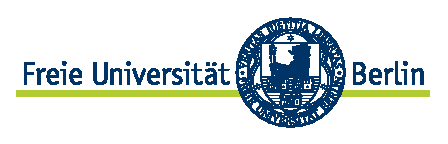
\includegraphics[width=0.4\textwidth]{src/fu_logo} % fügt FU-Logo ein
}
% /////////////////////// END TITLEPAGE /////////////////////////

\vspace{7cm}							% Abstand
\rule{\linewidth}{0.8pt}				% horizontale Linie

% /////////////////////// Task 1 /////////////////////////
\section{Recherche Softwarearchitektur}
\begin{enumerate}[(a)]
    % /////////////////////// a /////////////////////////
    \item {\itshape \textbf{Architekturebenen:}}
    \begin{itemize}
        \item {\itshape Welche gibt es, wodurch zeichnen sie sich jeweils aus.}
        \begin{itemize}
            \item \textbf{Organisationsebene:}
            \begin{itemize}
                \item Auf dieser Architektur-Ebene werden Organisationen (z. B. Unternehmen oder Institutionen), deren \textbf{Bebauungspläne, Geschäftsprozesse und IT-Landschaften} sowie deren Interaktionen mit anderen \textbf{Organisationen} betrachtet.(Seite 80, Absatz 1)
                \item Des Weiteren liegen im Kontext der Organisationsebene Anforderungen an eine Organisation sowie organisationsweit zu verwendende \textbf{IT-Standards und -Richtlinien}.(80,2)
                \item Insbesondere bei folgenden \textbf{Problemfeldern} wird sich ein Architekt auch auf der Organisationsebene bewegen müssen: (80,3)
                \begin{itemize}
                    \item IT-gestützte Umsetzung organisationsübergreifender Prozesse (z. B. Supply Chain Management).
                    \item Enterprise-Architektur.
                    \item Enterprise Application Integration (EAI)
                \end{itemize}
            \end{itemize} 


            
            \item \textbf{Systemebene:}
            \begin{itemize}
                \item Auf der Systemebene werden die \textbf{IT-Systeme von Organisationen} betrachtet. Der innere Aufbau der Systeme spielt hier nur in Bezug auf deren Subsysteme eine Rolle.(81,1) 
                \item Die \textbf{wesentlichen Elemente} auf der Systemebene sind: (81,1)
                \begin{itemize}
                    \item Anforderungen an die Systeme
                    \item Systemkontexte der Systeme
                    \item Subsysteme der Systeme
                \end{itemize}
            \end{itemize}
         
            
            \item \textbf{Bausteinebene:}
            \begin{itemize}
                \item Hier betrachtet man die Bausteine der Systeme.(73,2)
                \item Auf der Bausteinebene im Bereich Makro-Architektur wird die \textbf{innere Struktur} der einzelnen Subsysteme betrachtet.(82,1)
                \item \textbf{Wesentliche Aspekte}, mit denen man sich auf der Bausteinebene beschäftigt, sind die Verantwortlichkeiten der Systembausteine, deren Schnittstellen sowie deren Interaktionen untereinander.(82,1)
            \end{itemize}
            
            
        \end{itemize}
        
        \item {\itshape Wozu dient ihre Unterscheidung?}
        \begin{itemize}
            \item Architektur-Probleme/-Aspekte werden passenden Ebenen zugeordnet und sind damit einfacher und einheitlicher zu handhaben [Brown et al. 1998].(74,2)
            \item Unterschiedliche Architektur-Probleme/-Aspekte werden nicht vermischt, sondern getrennt mit den jeweils probaten Mitteln behandelt.(74,2)
            \item Einflüsse auf eine Architektur liegen explizit vor und können deshalb besser verstanden und berücksichtigt werden.(74,2)



        \end{itemize}
        
        
        \item {\itshape Was verstehen die Autoren unter einem „Ebenenwechsel“?}
        \begin{itemize}
            \item \textbf{Ebenenwechsel:} Bei sehr großen Systemen kann es sich bei den Systembausteinen, die sich aus der Dekomposition eines Subsystems ergeben haben, wiederum um Subsysteme anstelle von Software-Bausteinen handeln. In diesem Fall findet ein Ebenenwechsel von der Baustein- zurück auf die Systemebene statt. Dort findet die weitere Behandlung des Systembausteins als System ausgehend vom Systemkontext usw. statt.  Dadurch erhält das Architektur-Ebenen-Modell an dieser Stelle einen rekursiven Charakter.(82,2)
        \end{itemize}
        
        \item {\itshape {Worin besteht der Unterschied zwischen Makroarchitektur und Mikroarchitektur?}}
        \begin{itemize}
            \item \textbf{Makro-Architektur:} (Software-Architektur, Grob-Entwurf) Makro-Architektur umfasst das Spektrum der Architektur-Ebenen, denen architektonisch relevante Elemente zugeordnet sind (Organisations- und Systemebene sowie den Teilbereich der Bausteinebene, auf dem sich tragende Systembausteine befinden). Diese befasst sich mit Aspekten wie Anforderungen, Entscheidungen und Strukturen auf einem hohen Abstraktionsniveau. Die Organisations- und Systemebene sowie der Teil der Bausteinebene, dem die tragenden Bausteine eines Systems zugeordnet sind, gehören zum Bereich der Makro-Architektur.(78,4)
            
            \item \textbf{Mikro-Architektur:} (Detail- oder Fein-Entwurf) Mikro-Architektur dagegen befasst sich mit Aspekten auf einem niedrigen Abstraktionsniveau. Dabei handelt es sich dann um Detail-Entwurf (Architektur im „Kleinen“) mit großer Nähe zum Quelltext ohne fundamentalen Einfluss auf eine Architektur. Zum Bereich Mikro-Architektur gehört der Teilbereich der Bausteinebene, auf dem sich die nichttragenden Systembausteine befinden.(78,5)
        \end{itemize}
        
        \item {\itshape Durch welches entscheidende Merkmal wird der Übergang gekennzeichnet?}
        \begin{itemize}
            \item Die Grenze zwischen Makro- und Mikro-Architektur kann nicht immer klar gezogen werden. Diese ist auch abhängig von der Sicht der jeweiligen Interessenvertreter und deshalb ein fließender Übergang.(78,3)

        \end{itemize}
        
    \end{itemize}
    
    
  

    % /////////////////////// b /////////////////////////
    \item {\itshape \textbf{Architektursichten:}}
    \begin{itemize}
        \item {\itshape Welche gibt es und wodurch zeichnen sie sich jeweils aus?}
        \begin{itemize}
        
            \item Es ist in Anlehnung an [Rozanski und Woods 2005], [Bredemeyer und Malan 2004] und [Larman 2002] zu empfehlen, zumindest folgende \textbf{grundlegende Architektur-Sichten} immer vorzusehen: (89,5)
            \begin{enumerate}[1.]
            
                \item \textbf{Konzeptionelle Sicht (Geschäftssicht):} Diese Architektur-Sicht beschreibt die Systembausteine und ihre Beziehungen untereinander, ohne auf Details wie z. B. Schnittstellen einzugehen. Sie ist dazu geeignet, eine Architektur nicht-technischen Interessenvertretern zu vermitteln.(90,1)
                
                \item \textbf{Logische Sicht:} Diese Architektur-Sicht beschreibt die Systembausteine und ihre Beziehungen untereinander im Detail. Dabei werden die Systembausteine und ihre Beziehungen respektive die Kommunikationsmechanismen genau spezifiziert. Dies geschieht im Hinblick auf die technische Realisierung. Damit richtet sich diese Architektur-Sicht an technische Interessenvertreter.(90,2)
            
                \item \textbf{Ausführungssicht (Verteilungssicht):} Diese Architektur-Sicht beschreibt im Detail die physikalische Verteilung der Systembausteine zur Laufzeit. Sie richtet sich ebenfalls an technische Interessenvertreter.(90,3)
            \end{enumerate}
            
            
            
            \item Als \textbf{grundlegende Architektur-Sichten} werden die Anforderungssicht, die logische Sicht, die Datensicht, die Umsetzungssicht, die Prozesssicht und die Verteilungssicht unterschieden. (101,5)
            \begin{enumerate}[1.]
                
                \item \textbf{Anforderungssicht:} beschreibt die Architektur-Anforderungen.(91,2)
                
                \item \textbf{Logische Sicht:} beschreibt die Dokumentation des Architektur-Entwurfs.(91,3)
                
                \item \textbf{Datensicht:} beschreibt die Aspekten bezüglich Speicherung, Manipulation,Verwaltung und Verteilung von Daten.(92,1)
                
                \item \textbf{Umsetzungssicht:} beschreibt die Umsetzungsstruktur und der Umsetzungsinfrastruktur.(92,2)
                
                \item \textbf{Prozesssicht:} beschreibt die Steuerung und Koordination nebenläufiger Bausteine.(92,3)
                
                \item \textbf{Verteilungssicht:} beschreibt die physikalische Verteilung von Software-Bausteinen..(93,2)
            \end{enumerate}
            

        \end{itemize}
        
        \item {\itshape Wozu dient ihre Unterscheidung?}
        \begin{itemize}
            \item Alle Aspekte komplexer Systeme (Menschen, Bauwerke, IT-Systeme etc.) zu jedem Zeitpunkt komplett zu erfassen, ist zumindest für die menschliche Wahrnehmung nicht möglich. Dies zu versuchen, wäre darüber hinaus auch nicht zielführend, weil nicht zu jedem Zeitpunkt gleichzeitig alle Aspekte eines Systems relevant sind. Daher ist es sinnvoll, nur bestimmte, für den Moment interessante Aspekte eines Systems betrachten zu können. Für IT-Systeme existiert zu diesem Zweck das Konzept der Architektur-Sichten.(83,1)

            \item Architektur-Sichtenmodellen umfassen alle relevanten Architektur-Sichten und ermöglichen es damit, Architektur überhaupt erst greifbar bzw. sichtbar zu machen. Die Komplexität der Architektur eines Systems kann erst durch Architektur-Sichtenmodelle bewältigt werden.(89,1)

            \item Mithilfe eines Architektur-Sichtenmodells lässt sich nachprüfen, ob eine Architektur wie gewünscht alle relevanten Aspekte eines Systems abdeckt. Wird eine Architektur gleich zu Beginn auf Basis eines Architektur-Sichtenmodells erstellt, verringert sich die Wahrscheinlichkeit, dass wichtige architekturrelevante Punkte vergessen und deshalb von der Architektur nicht gewürdigt werden.(89,4)
            
            \item Mittels Architektur-Sichten lassen sich gezielt bestimmte Aspekte eines IT-Systems betrachten. Damit verhelfen Architektur-Sichten dazu, mit der Komplexität aller Aspekte eines IT-Systems einfacher umzugehen.(101,1)


        \end{itemize}
        
    \end{itemize}
   

    % /////////////////////// c /////////////////////////
    \item {\itshape \textbf{Architekturstile}: Welche gibt es und wodurch zeichnen sie sich aus?}
   \begin{itemize}
       \item Ein Architektur-Stil gibt in erster Linie die fundamentale Struktur eines Software-Systems und dessen Eigenschaften wieder. Ein Stil kann also genutzt werden, um Architekturen zu kategorisieren. Ferner kann man Stile dazu verwenden, um die Konsequenzen einer fundamentalen Architektur und ihrer Varianten zu verstehen.(199,4) (Bsp. Pipes-and-Filters-Architektur.)

        \item Ein Architektur-Stil besteht bei Shaw und Garlan aus den folgenden Elementen: 
        \begin{enumerate}[1.]
           \item Eine Menge von Komponententypen, die bestimmte Funktionen zur Laufzeiterfüllen.(199,2)
           \item Eine topologische Anordnung dieser Komponenten.(199,2)
           \item Eine Menge von Konnektoren, die die Kommunikation und Koordination zwischen den Komponenten regeln.(199,2)
           \item Eine Menge von semantischen Einschränkungen, die bestimmen, wieKomponenten und Konnektoren miteinander verbunden werden können.(199,2)
       \end{enumerate}
   \end{itemize}
    
\end{enumerate}

% /////////////////////// Task 2 /////////////////////////
\section{Architekturstile}
\begin{enumerate}[(a)]
    % /////////////////////// a /////////////////////////
    \item {\itshape Nennen Sie zu jedem der in der Vorlesung genannten Architekturstile ein Ihnen bekanntes Softwaresystem, das diesen Stil verwendet. Woran erkennen Sie das jeweils? (Nehmen Sie nicht die auf den Folien schon genannten Beispiele.)}
    \begin{enumerate}[1.]
        \item \textbf{Client / Server-Architektur:}
        \begin{itemize}
            \item Beispiel \textbf{Email}:
            \item Es gibt einen zentralen Rechner (Server), welcher die Daten (Emails) speichert.
            \item Es gibt zahlreiche Klienten, welche die Daten abfragen und gegeben falls weitere Aktivitäten von dem Server beanspruchen (Versenden usw.)
        \end{itemize}
        
        \item \textbf{Schichten-Architektur:}
        \begin{itemize}
            \item Beispiel \textbf{Betriebssystem}
            \item Es gibt mehrere Schichten (Ringe) und höhere Schichten werden von niederen niemals benutzt.
            \item Ring 0 $\xrightarrow{}$ Kernel, Ring 1 $\xrightarrow{}$ Executive, Ring 2 $\xrightarrow{}$ Supervisor, Ring 3 $\xrightarrow{}$ User
        \end{itemize}
        
        \item \textbf{Architekturstil Ereignisgesteuerung:}
        \begin{itemize}
            \item Beispiel \textbf{Windows Ereignis Manager}
            \item Es werden auf Ereignisse gelauscht und man wird benachrichtigt, falls eins Eintritt.
            \item Man kann selbst Ereignisse erstellen.
        \end{itemize}
        
        \item \textbf{Architekturstil Datenflussnetze (Pipes und Filter):}
        \begin{itemize}
            \item Beispiel \textbf{Email}
            \item Vom senden einer Email, zur verschlüsselung im Server bis zum ankommen beim Adressaten muss eine Email oft bearbeitet werden. Dies kann mithilfe von Pipes und von Filter dargestellt werden.
            \item 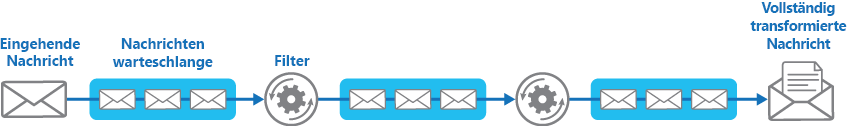
\includegraphics[width=0.9\textwidth]{src/u7/pipes-and-filters-message-queues.png}[6]
        \end{itemize}
        
        \item \textbf{Standartarchitektur: Web-basiertes System:}
        \begin{itemize}
            \item Beispiel \textbf{Mobile API}
            \item Creating these services have become easier using simplified web protocols, e.g. REST and JSON.[2]
            \item These protocols are much easier for web developers, as they require less CPU and bandwidth. They are more recognised because of large social platforms, such as Facebook, Amazon and Twitter etc.[2]
            
        \end{itemize}
        
    \end{enumerate}
    
    
    % /////////////////////// b /////////////////////////
    \item {\itshape Welche Architekturstile sind für welche der folgenden nicht-funktionalen Anforderungen besonders geeignet?}

    \begin{enumerate}[1.]
        \item {\itshape \textbf{Echtzeitverhalten} (d.h. zugesicherte Reaktionszeiten des Systems)}  
        \begin{itemize}
            \item Datenflussnetze (in der VL als Bsp Bioinformatik und Signalverarbeitung).
        \end{itemize}
        
        \item {\itshape \textbf{hohe Portabilität} (über mehrere Betriebssystemplattformen)}
        \begin{itemize}
            \item Client-Server Architektur, Web-basierte Architektur. Also im Prinzip die Architekturen, welche nur wenig auf das Betriebssystem ankommen. 
        \end{itemize}
    \end{enumerate}

\end{enumerate}

% /////////////////////// Task 3 /////////////////////////
\section{Architekturbeschreibung Ihres Softwareprojektes}
\begin{enumerate}[(a)]
    % /////////////////////// a /////////////////////////
    \item {\itshape In Aufgabe7-1sollten Sie dem4+1-Sichtenmodellvon Kruchten begegnet sein. Ma-chen Sie sich soweit mit diesem Modell vertraut, dass Sie den Zweck der einzelnenSichten  verstehen.}
    
    % /////////////////////// b /////////////////////////
    \item {\itshape Entwerfen Sie die Architektur Ihres Softwaresystems. Nehmen Sie dabei die folgendenSichten ein und halten Sie jeweils mindestens drei wichtige Aspekte fest. Sollte IhrSystem aus einer der Sichten keine relevante Architektur haben, erläutern Sie dies.}

    \begin{enumerate}[1.]
        \item Anwendungsfallsicht(use-case view/scenarios) \\
        Die Anwendungsfallsicht umfasst die wichtigsten Anwendungsfälle, also geben wir für die Aufgabe drei wichtige Anwendungsfälle vor.
        Unserer Meinung nach sind die 3 wichtigsten Anwendungsfälle die folgenden:\\
        1. Quittung Scannen \\
        2. Scan vorbereiten \\
        3. Quittung in der App suchen (aus Übung 5) \\
        
         \begin{tabular}{l|l}
            Anwendungsfall &  1.User\_Scan\_Receipt \\ 
            \hline  
            Beschreibung & Benutzer scannt eine Quittung. \\
            \hline  
            Akteure & Benutzer und App \\
            \hline  
            Annahmen & Handy hat Kamera \\
            \hline  
            Schritte & 1. Benutzer öffnet App. \\
            & 2. Benutzer klickt auf den Button zum Scannen einer Quittung. \\
            & 3. App öffnet Kamera-Ansicht \\
            & 4. Benutzer scannt QR-Code \\
            & 5. App erkennt QR-Code und schließt App\\
            \hline  
            Variationen &  \\
            \hline  
            Nicht-funktionales & Keine \\
            \hline  
            Probleme &  \\
            \hline  
 
        \end{tabular}
        
        
        \begin{tabular}{l|l}
            Anwendungsfall &  User\_Prepare\_Scan \\ 
            \hline  
            Beschreibung & Kassierer bereitet einen Scan vor. \\
            \hline  
            Akteure & Kassierer, Kunde und App \\
            \hline  
           Annahmen & Kasse hat einen Scan Button \\
            \hline  
            Schritte & 1. Kassierer öffnet App. \\
            & 2. Benutzer klickt auf den Button zur Vorbereitung eines Scans. \\
            & 3. Display zeigt QR-Code \\
            & 4. Kunde scannt QR-Code \\
            & 5. App erkennt QR-Code, \underline{speichert es in die Datenbank} und schließt App\\
            \hline  
            Variationen &  \\
            \hline  
            Nicht-funktionales & Keine \\
            \hline  
            Probleme &  \\
            \hline  
 
        \end{tabular}

         \begin{tabular}{l|l}
            Anwendungsfall & 3. User\_Searchs\_Receipt \\ 
            \hline  
            Beschreibung & Benutzer sucht eine Quittung. \\
            \hline  
            Akteure & Benutzer und App \\
            \hline  
            Annahmen & Quittung ist in der App vorhanden. \\
            \hline  
            Schritte & 1. Benutzer öffnet App. \\
            & 2. Benutzer klickt auf den Button zum Suchen einer Quittung. \\
            & 3. App öffnet ein Dialog mit Filter für die Suche. \\
            & 4. Benutzer trägt benötigte Daten ein: Datum/Zeitraum, Kategorie, Markt \\
            & 5. Benutzer bestätigt seine Eingaben. \\
            & 6. App schließt Dialog und zeigt alle Quittungen mit diesem Filter an. \\
            \hline  
            Variationen & \#4. Benutzer kann Daten weglassen \\
            & \#5. Benutzer bestätigt nicht und schließt den Dialog, alles bleibt so wie es ist. \\
            \hline  
            Nicht-funktionales & Keine \\
            \hline  
            Probleme & Falls Quittungen online gespeichert sind und kein Internetzugang besteht, \\ 
            & werden die Quittungen nicht angezeigt. \\
            \hline  
 
        \end{tabular}
        
        
        
        \item Logische Sicht(logical view)\\
        Aus der logischen Sicht, wird die Umsetzung der funktionalen Anforderungen betrachtet. Dabei werden UML-Diagramme zur Darstellung benutzt.
        In unserem Beispiel haben wir ein UML-Klassendiagramm benutzt um die in der Anwendungsfallsicht genannten funktionalen Anforderungen mithilfe eines Klassendiagramms darzustellen.\\
        1. Unsere App soll sich mit der Datenbank verbinden können. \\
        2. Unsere App soll es den Kunden ermöglichen die Quittungen zu suchen und zu scannen. \\
        3. Unsere App soll es den Kassierern ermöglichen den Scan vorzubereiten. \\
        \begin{itemize}
        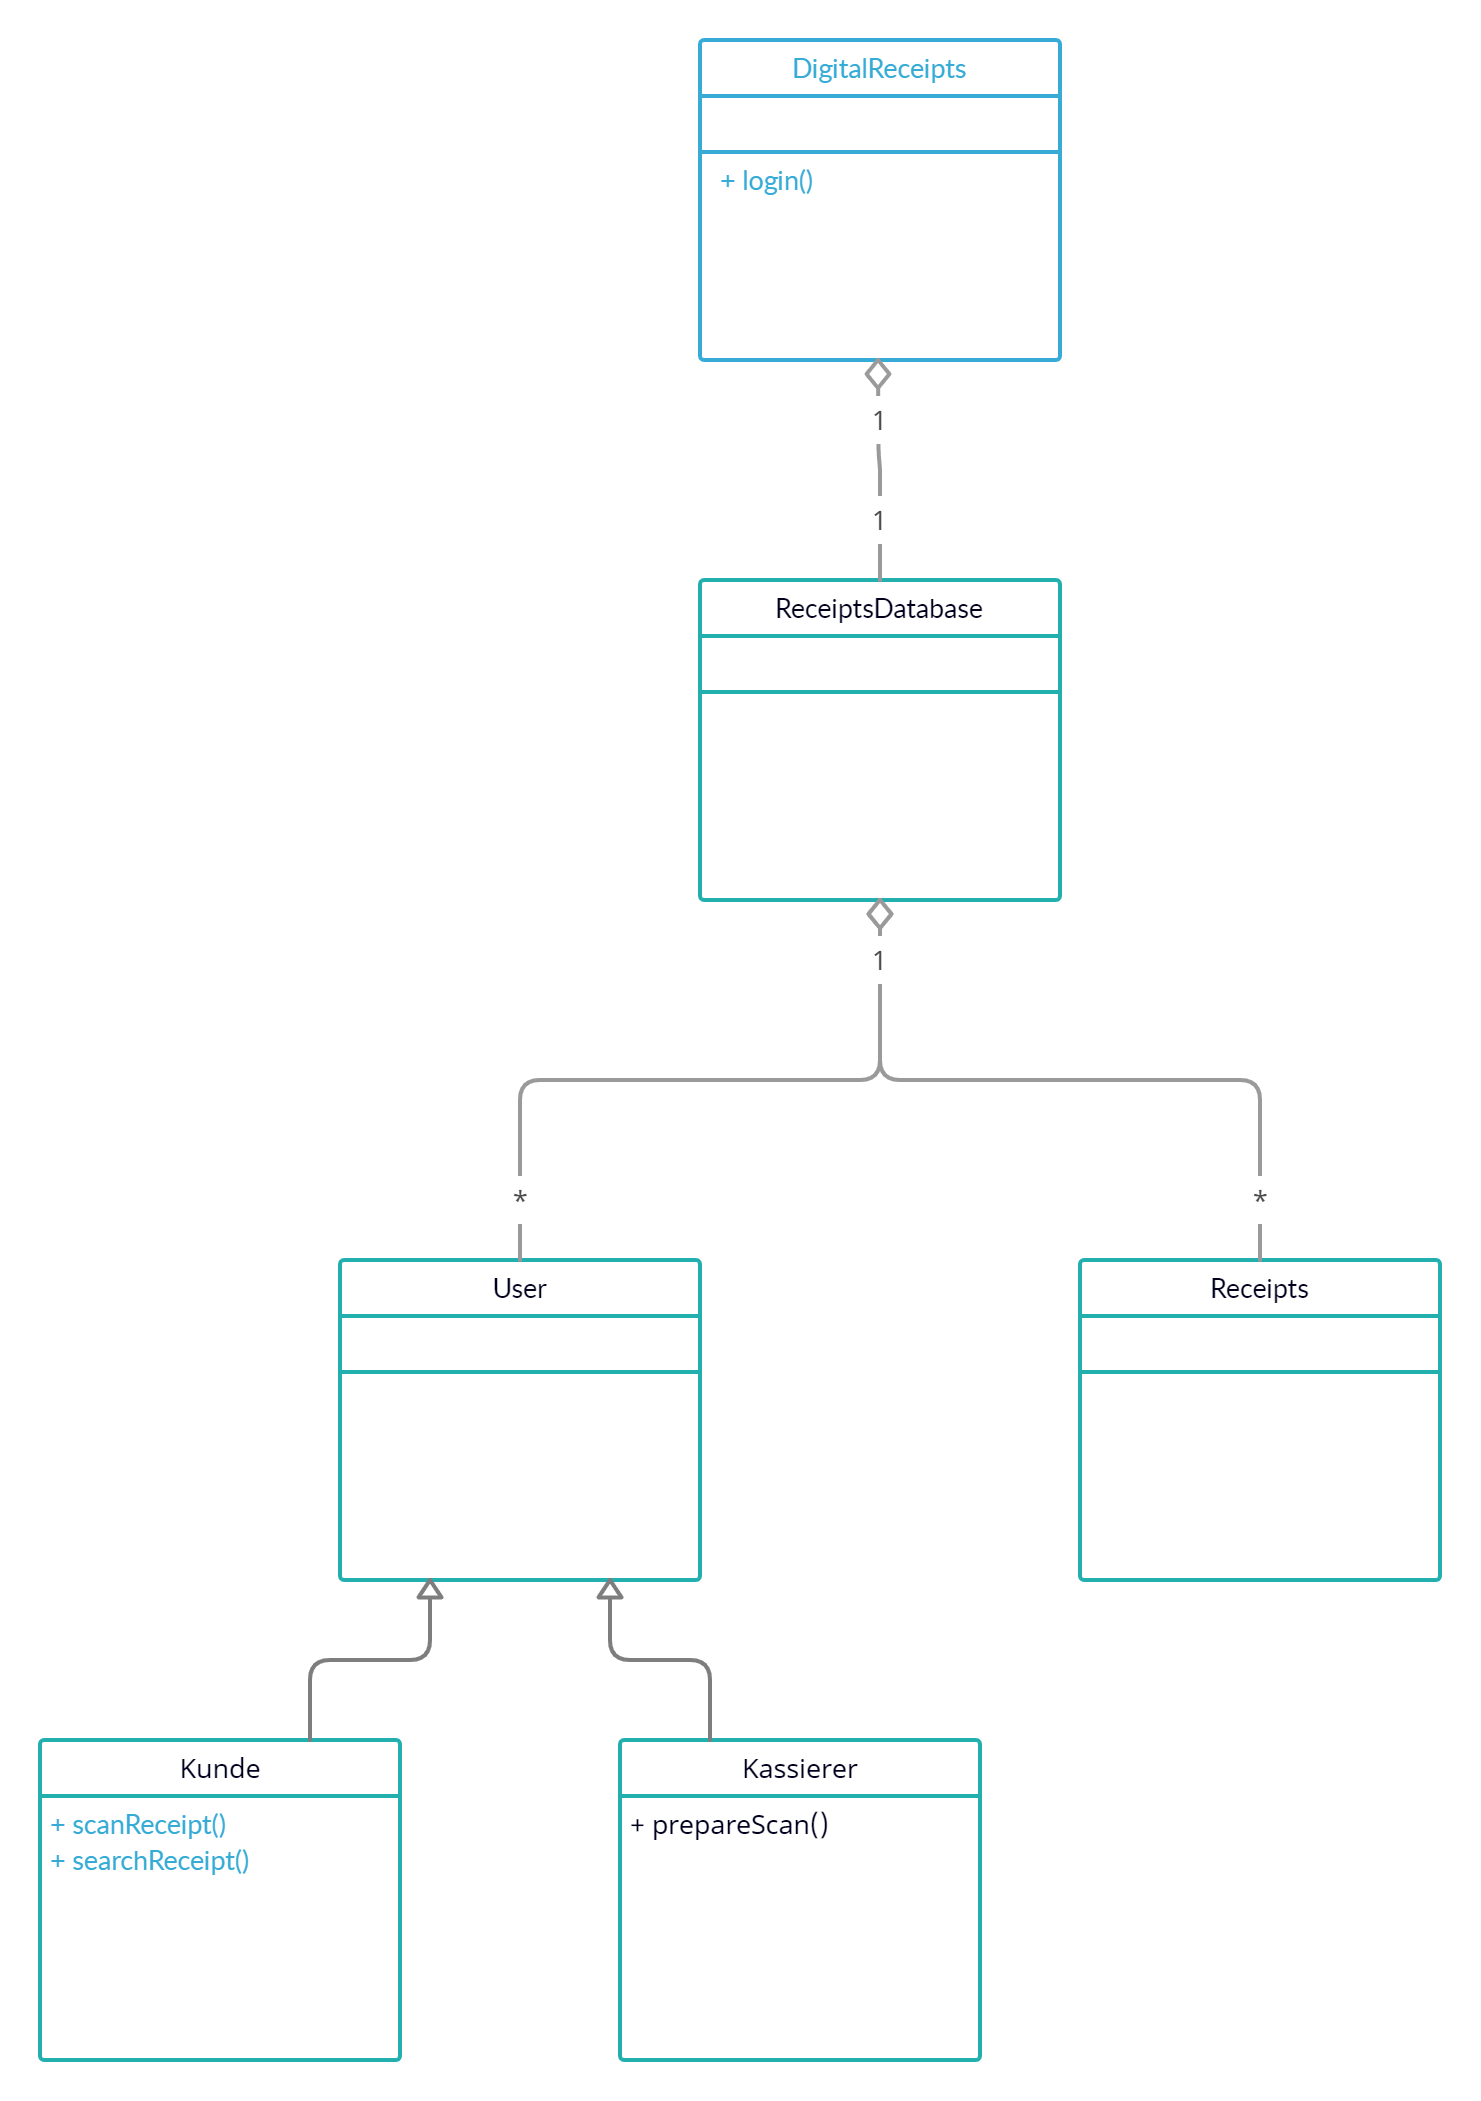
\includegraphics[width=12cm,height=12cm,keepaspectratio]{src/u7/Class_Diagram_7.png}
         \end{itemize} 
        Anmerkung: DigitalReceipts soll die Benutzeroberfläche darstellen.
        
        \item Implementierungssicht(implementation view/development view)\\
        Die Implementierungsschicht behandelt die Organisation und Verwaltung der Software (Softwaremanagement).\\
        Eine gute Verwaltung/Organisation schaffen wir mithilfe der Modularisierung, damit wir einen guten Überblick über unsere Software und ihre Einzelheiten haben.\\
        1. Die Benutzeroberfläche ist lokal gespeichert.\\
        2. Die App ist die Schnittstelle zum Server.\\
        3. Bevor man zugriff zum Server hat muss man sich Authentifizieren (login).\\
        Hier haben wir uns an die Pipe-and-Filter-Architektur aus der Vorlesung gehalten um das ganze einfach zu modellieren:
        \begin{itemize}
        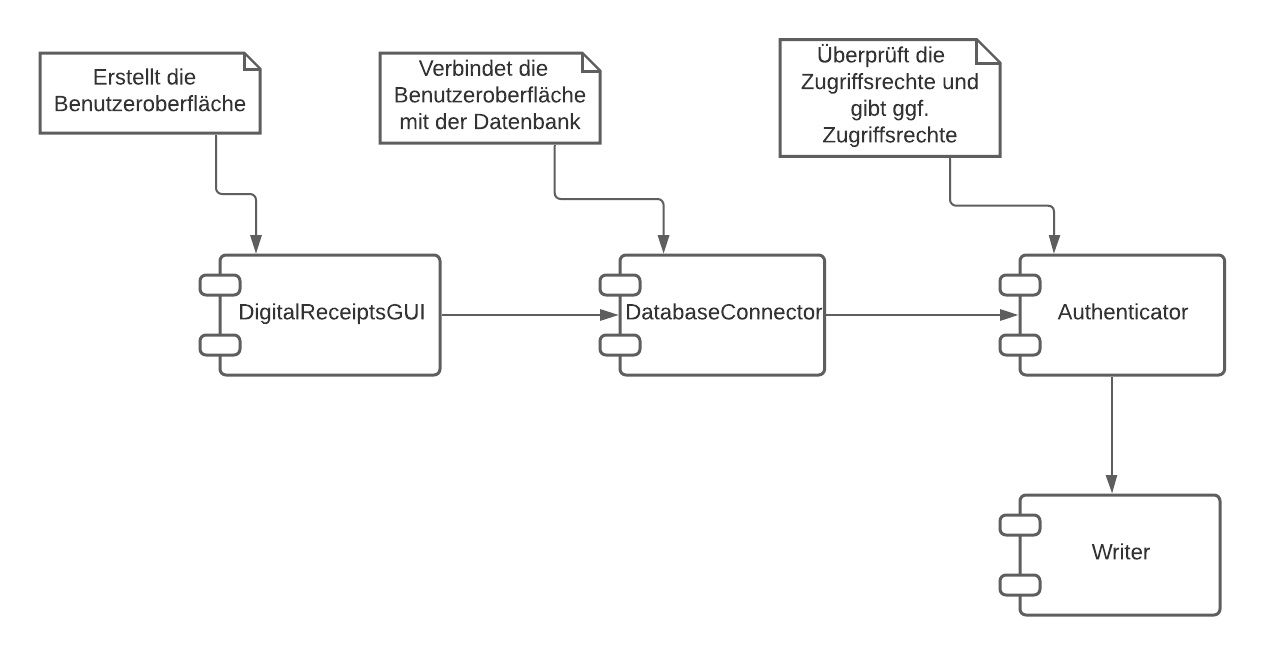
\includegraphics[width=15cm,height=15cm,keepaspectratio]{src/u7/Component_7.png}
         \end{itemize} 
        \item Prozesssicht (process view) \\
        Die Prozesssicht behandelt das Verhalten und Verteilung des Systems zur Laufzeit, da unser System auf mehreren Systemen läuft können wir das am besten mit einem Aktivitätsdiagramm modellieren.
        Hier haben wir unser wichtigste Funktion modelliert:\\
        1. Um eine digitale Quittung zu Scannen muss der Kassierer erst den Scan vorbereiten. \\
        2. Erst nach dem der Scan vorbereitet wurde kann man die digitale Quittung in form eines QR Code scannen. \\
        3. Erst dann wird die Quittung in die Datenbank gespeichert. \\
        \begin{itemize}
        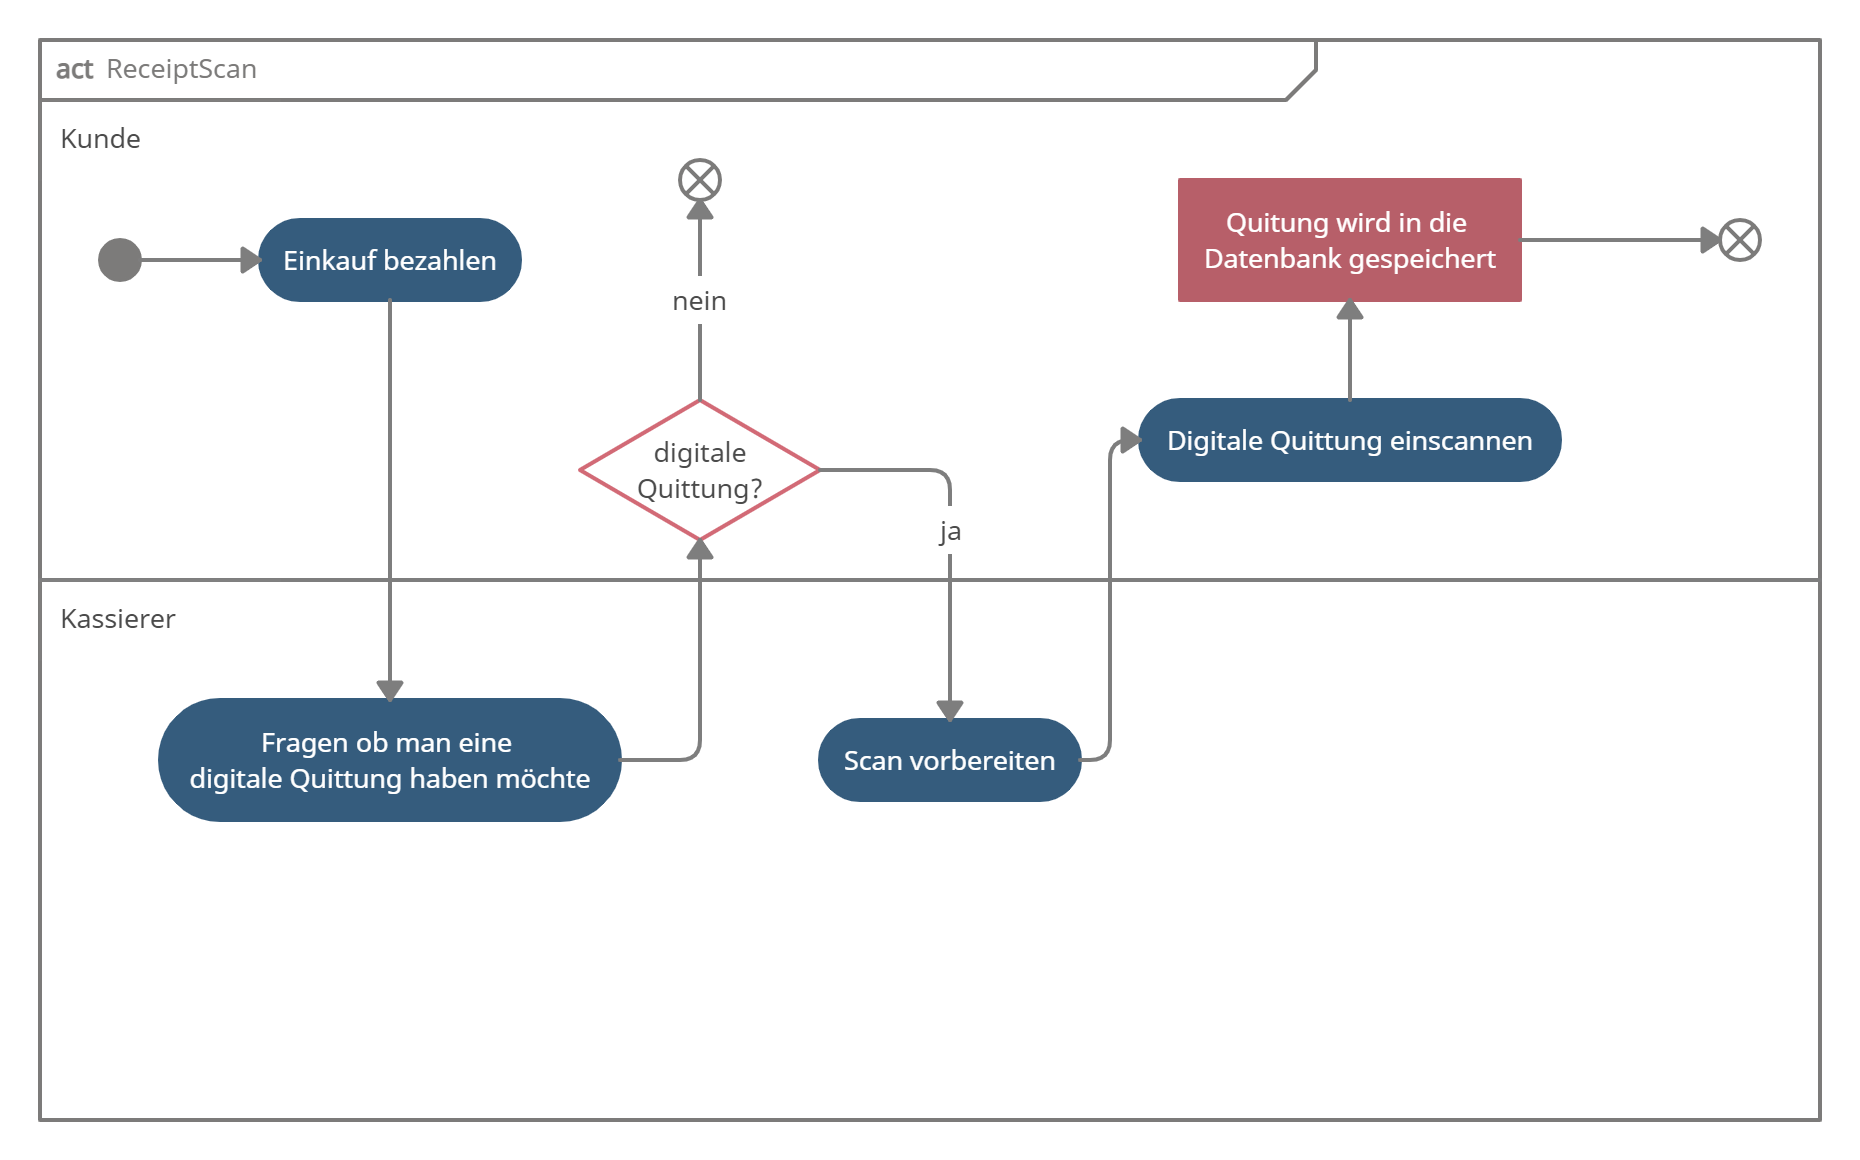
\includegraphics[width=15cm,height=15cm,keepaspectratio]{src/u7/Activity_7.png}
         \end{itemize} 
        
        \item Verteilungssicht (deployment view/physical view) \\
        Die Verteilungssicht behandelt, wie die Implementierungssicht physikalisch umgesetzt werden kann.
        1. Die App stellen wir im App Store und im Play Store zur Verfügung. \\
        2. Die App stellt eine verschlüsselte Verbindung zum Server her über das Internet her. \\
        3. Die Quittungen sind alle auf dem Server gespeichert, damit man die nicht fälschen kann. \\
    \end{enumerate}

\end{enumerate}


\section{Quellen}
\begin{enumerate}[{[1]}]
    \item  \textbf{Für Aufgabe 1:} ``Webbasierte Systemarchitekturen'', \url{https://link.springer.com/chapter/10.1007%2F978-3-322-89822-7_4} .
[aufgerufen am 29.05.2021]
    \item ``Web-oriented architecture'', \url{https://en.wikipedia.org/wiki/Web-oriented_architecture} [aufgerufen am 29.05.2021]
    \item \textbf{Für Aufgabe 3:} "4+1 Schichtenmodell",
    \url{https://de.wikipedia.org/wiki/4%2B1_Sichtenmodell} [aufgerufen am 29.05.2021]
    \item "The 4+1 View Model of Architecture",
    \url{https://de.wikipedia.org/wiki/4%2B1_Sichtenmodell} [aufgerufen am 29.05.2021]
        \item "SoftwareArchitektur",
    \url{https://link.springer.com/book/10.1007/978-3-8274-2267-5} [S.98-99]
    
    \item ``Muster „Pipes und Filter'', \url{https://docs.microsoft.com/de-de/azure/architecture/patterns/pipes-and-filters}, [aufgerufen am 29.05.2021]
\end{enumerate}


\end{document}